\section{Machine Learning Classifier}
Classifier is a type of machine learning algorithm used to assign a class label to a data input. Classifier algorithms are trained using labeled data; in the image recognition example, for instance, the classifier receives training data that labels images. After sufficient training, the classifier then can receive unlabeled images as inputs and will output classification labels for each image.\par \vspace{1em}

% Classifier algorithms employ sophisticated mathematical and statistical methods to generate predictions about the likelihood of a data input being classified in a given way. In the image recognition example, the classifier statistically predicts whether an image is likely to be a car, a truck, or a person, or some other classification that the classifier has been trained to identify.

    \subsection{ConvNet Models}
        
        \subsubsection{VGG16}
        \begin{figure}
            \centering
            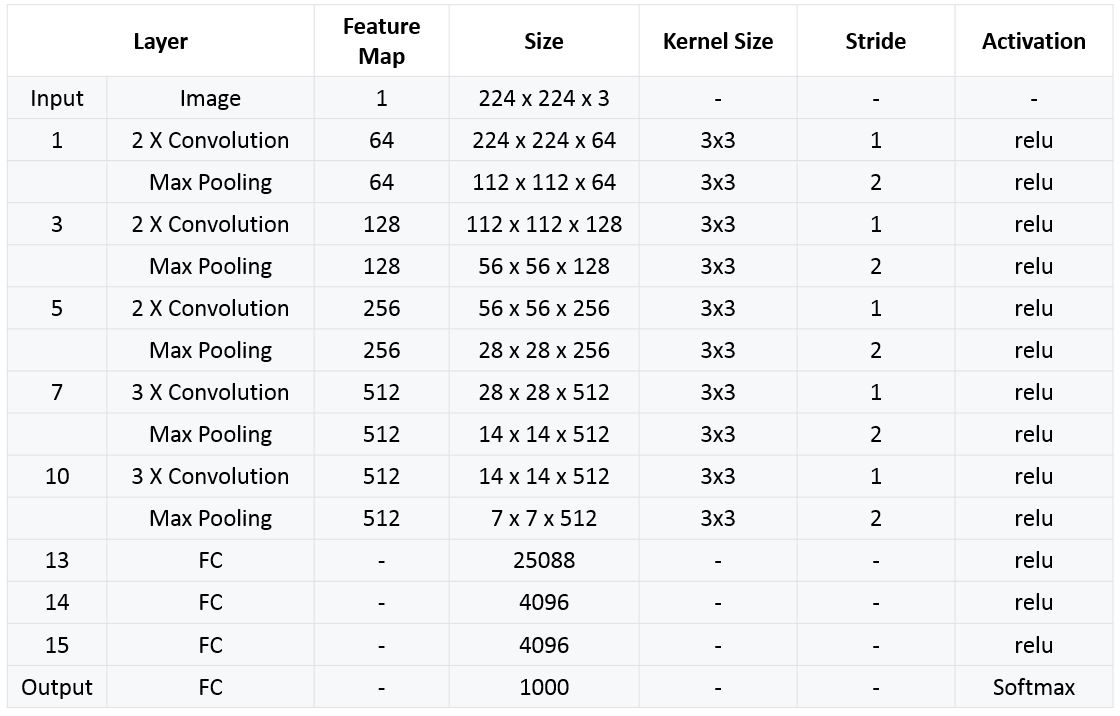
\includegraphics[width=1\linewidth]{graphics//chapter3/vgg16 arch.png}
            \caption{VGG16 Architecture, Source: \cite{WEBSITE:vgg16-arch-diagram}}
            \label{fig:vgg16-arch}
        \end{figure}
        
        VGG16 is a deep convolutional neural network model used for image classification tasks. The network is composed of 16 layers of artificial neurons, which each work to process image information incrementally and improve the accuracy of its predictions.\par \vspace{1em}

        VGG16 uses convolution layers with a 3x3 filter and a stride 1 that are in the same padding and maxpool layer of 2x2 filter of stride 2. It follows this arrangement of convolution and max pool layers consistently throughout the whole architecture. In the end it has two fully connected layers, followed by a softmax for output\cite{vgg16}.\par \vspace{1em} 

        In VGG16, ‘VGG’ refers to the Visual Geometry Group of the University of Oxford, while the ‘16’ refers to the network’s 16 layers that have weights.
        
        \subsubsection{MobileNetV2}
        
        \begin{figure}[h]
            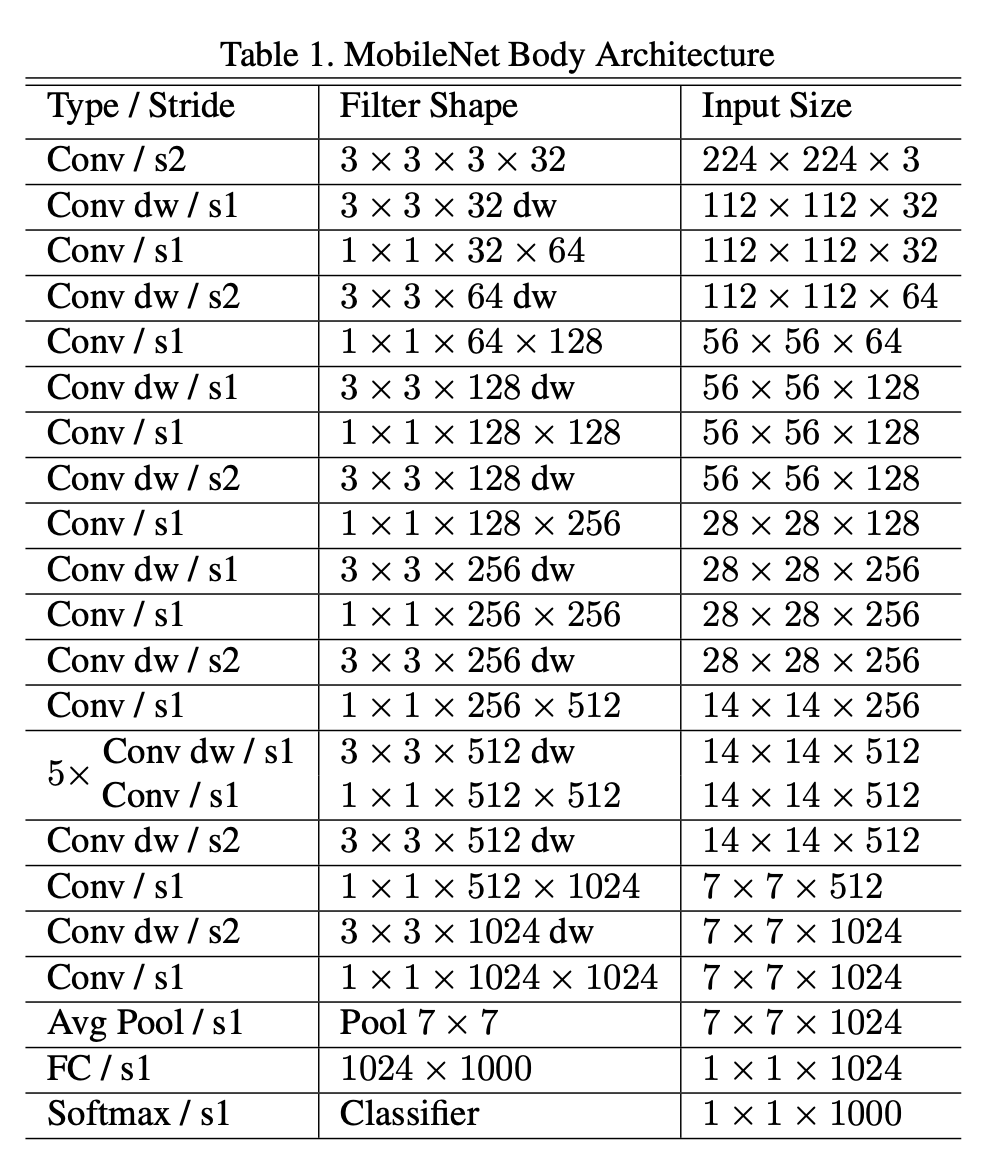
\includegraphics[width=0.5\textwidth, center]{graphics/chapter3/mobnetV1.png}
            \caption{MobileNetV2 Block Diagram, Source: \cite{mobilenetV1}}
            \label{fig:MobileNetV2Block}
        \end{figure}

        \begin{figure}[h]
            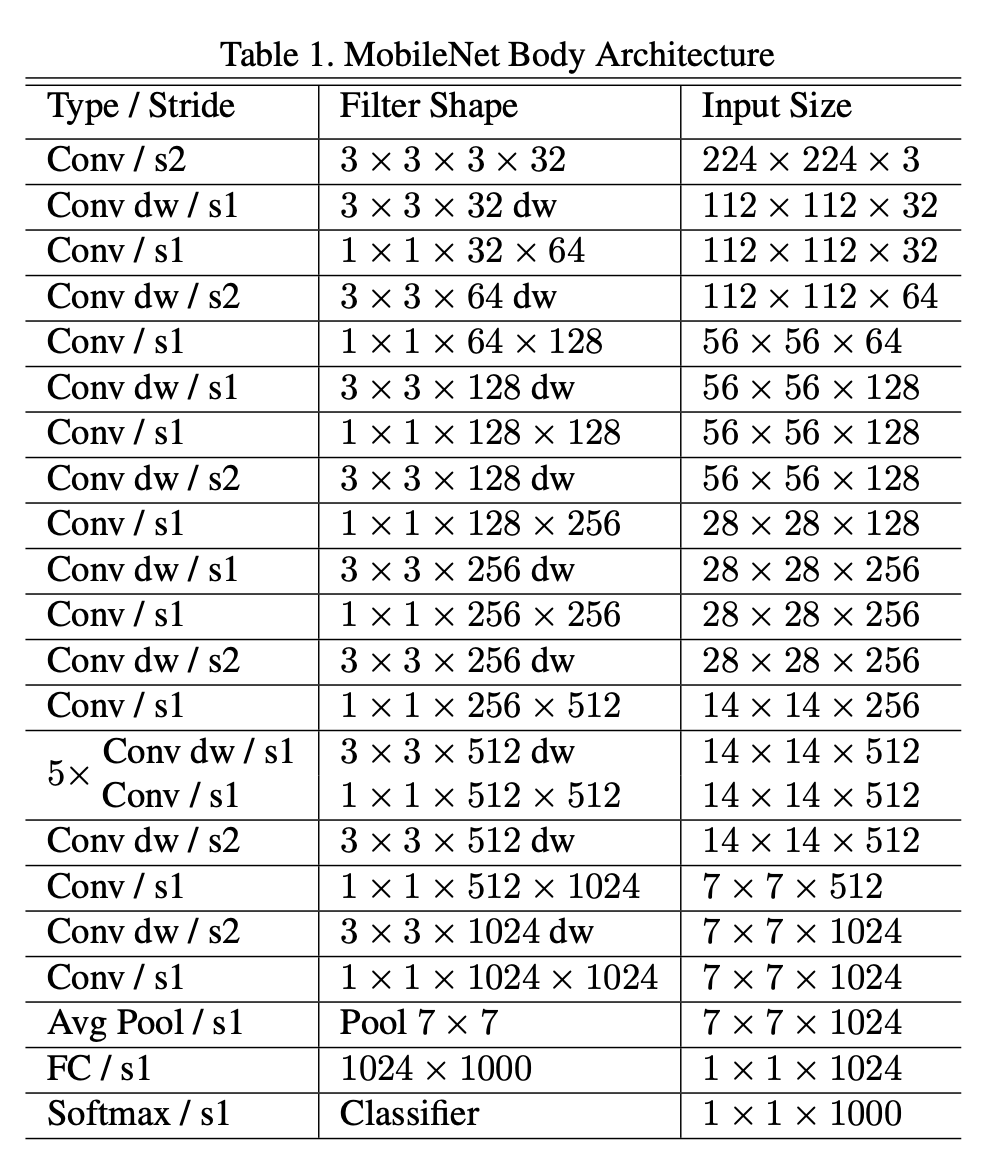
\includegraphics[width=0.5\textwidth, center]{graphics/chapter3/mobnetV1.png}
            \caption{MobileNetV2 Architecture, Source: \cite{mobilenetV1}}
            \label{fig:MobileNetV2}
        \end{figure}
        
        MobileNetV2, is a lightweight convolutional neural network (CNN) architecture, specifically designed for mobile and embedded vision applications. Google researchers developed it as an enhancement over the original MobileNet model. A remarkable aspect of this model is its ability to strike a good balance between model size and accuracy, rendering it ideal for resource-constrained devices \cite{mobilenetV1}.\par \vspace{1em}

        MobileNetV2 architecture incorporates several key features that contribute to its efficiency and effectiveness in image classification tasks. These features include depthwise separable convolution, inverted residuals, bottleneck design, linear bottlenecks, and squeeze-and-excitation (SE) blocks\cite{mobilenetV2}. Each of these features plays a crucial role in reducing the computational complexity of the model while maintaining high accuracy.
        
        \subsubsection{Xception} 
        \begin{figure}
            \centering
            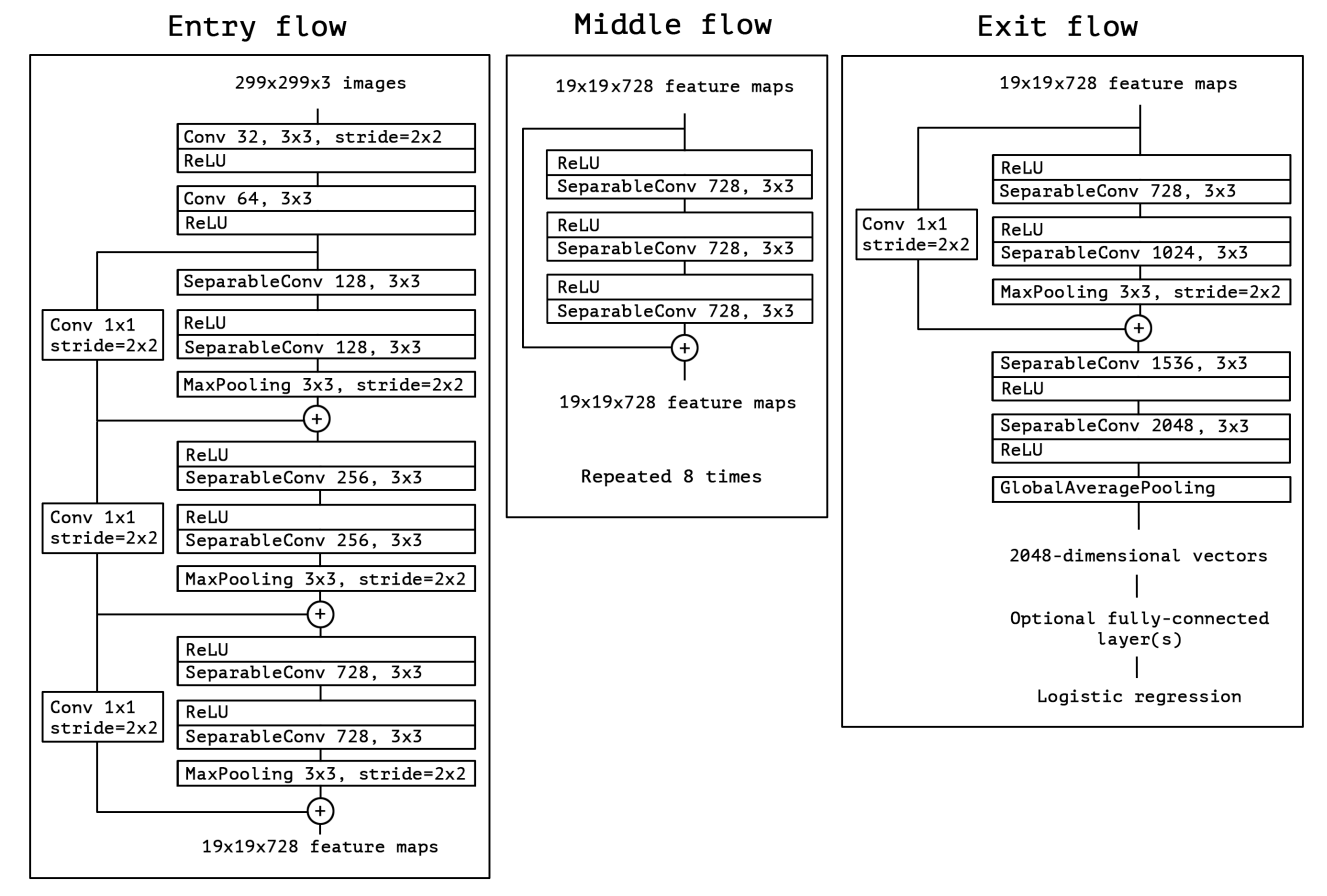
\includegraphics[width=1\linewidth]{graphics//chapter3/xception arch.png}
            \caption{Xception Architecture, Source: \cite{xception}}
            \label{fig:xception-arch}
        \end{figure}
        
        Xception is a deep convolutional neural network architecture that involves Depthwise Separable Convolutions. It was developed by Google researchers. Google presented an interpretation of Inception modules in convolutional neural networks as being an intermediate step in-between regular convolution and the depthwise separable convolution operation (a depthwise convolution followed by a pointwise convolution)\cite{xception}. \par \vspace{1em}
        
        In this light, a depthwise separable convolution can be understood as an Inception module with a maximally large number of towers. This observation leads them to propose a novel deep convolutional neural network architecture inspired by Inception, where Inception modules have been replaced with depthwise separable convolutions.\par \vspace{1em}

        Xception is an efficient architecture that relies on Depthwise Separable Convolution and Shortcuts between Convolution blocks as in ResNet.
        

    \subsection{CNN10L - Scratch Model}
    CNN10L (short 10 Convolutional layer model) is ConvNet Model built by our team.
    It's composed of \textit{10 convolutional layers, 3 max pooling layers, 2 Dense Layers, 1 Global Average 2D Pooling Layers and 1 Dropout Layer}. The Layer architecture is shown in figure \ref{fig:CNN10L}. We used non-linear activation function ReLu in each of the output of convolutional layer. \par\vspace{1em}
    The model is designed in such a way that there is balance in depth and width of feature learned.
    Our aim is to check whether such a shallow model can perform on par with famous very deep convnet model like VGG16, Xception, etc on narrow domain of plant disease detection tasks. Our main emphasis is also to reduce the computational power used by the model by developing a shallow model. And also by training our model from scratch and others by transfer learning, we can check how features learned from larger datasets like \textbf{ImageNet} contribute significantly to improving performance and efficiency when training on narrower domain tasks.
    \par\vspace{1em}
    A detailed description of the model with its input shape and output shape is also given in figure \ref{fig:cnn10l-detail-arch}.\par\vspace{1em}

    \begin{figure}[h]
        \centering
            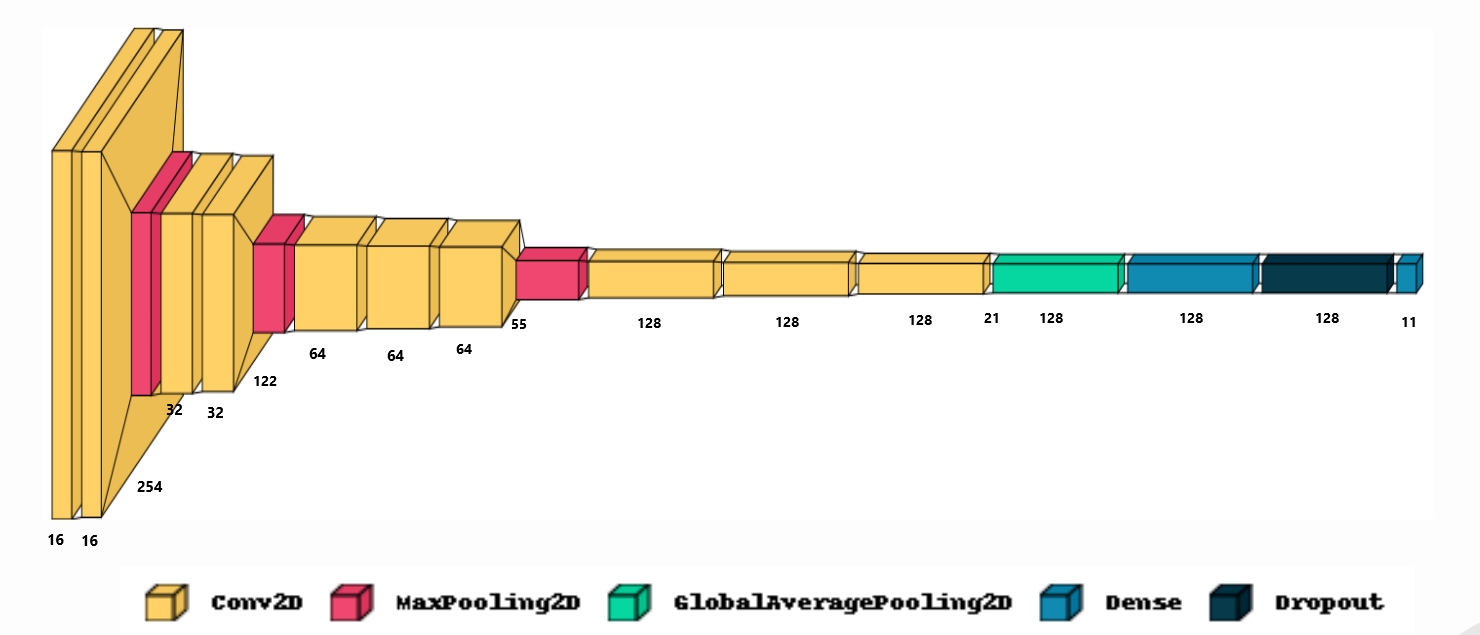
\includegraphics[width=\textwidth]{graphics/chapter3/CNN10L with label.png}
            \caption{CNN10L Architecture}
            \label{fig:CNN10L}
    \end{figure}

    \begin{figure}
        \centering
        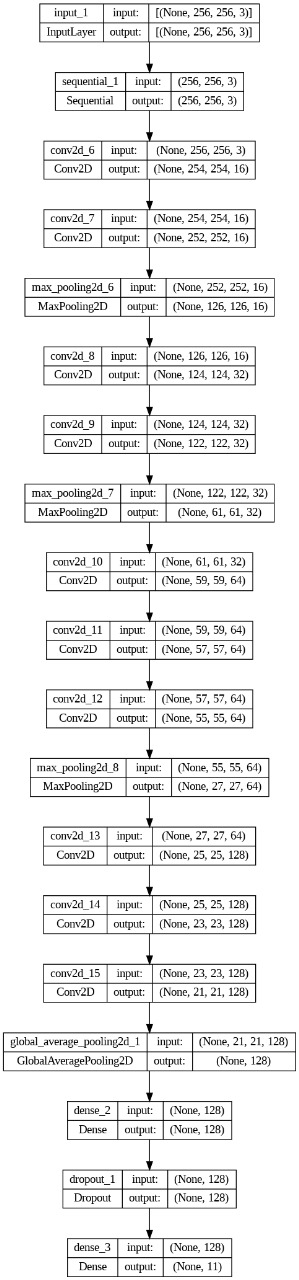
\includegraphics[height=\textheight]{graphics//chapter3/cn10oiedwf.jpg}
        \caption{CNN10L Detail Architecture}
        \label{fig:cnn10l-detail-arch}
    \end{figure}

    \begin{table}[h]
    \centering
    \begin{tabular}{cccc}
        \toprule
        \textbf{Type/Stride} & \textbf{Filter Shape} & \textbf{Input Size} & \textbf{Output Size}\\
        \hline
        \textbf{conv2d / s1} & \textbf{3 x 3 x 16}  & \textbf{3 x 3 x 16} & \textbf{254 x 254 x 3 x 16}\\
        \hline
        \textbf{conv2d / s1} & \textbf{3 x 3 x 16}  & \textbf{254 x 254 x 16} & \textbf{252 x 252 x 16}\\
        \hline
        \textbf{max\_pool / s2} & \textbf{2 x 2}  & \textbf{252 x 252 x 16} & \textbf{126 x 126 x 16}\\
        \hline
        \textbf{conv2d / s1} &\textbf{3 x 3 x 32}  & \textbf{126 x 126 x 16} & \textbf{124 x 124 x 32}\\
        \hline
        \textbf{conv2d / s1} &\textbf{3 x 3 x 32}  & \textbf{124 x 124 x 32} & \textbf{122 x 122 x 32}\\
        \hline
        \textbf{max\_pool / s2} & \textbf{2 x 2}  & \textbf{122 x 122 x 32} & \textbf{61 x 61 x 32}\\
        \hline
        \textbf{conv2d / s1} & \textbf{3 x 3 x 64}  & \textbf{61 x 61 x 32} & \textbf{59 x 59 x 64}\\
        \hline
        \textbf{conv2d / s1} & \textbf{3 x 3 x 64}  & \textbf{59 x 59 x 64} & \textbf{57 x 57 x 64}\\
        \hline
        \textbf{conv2d / s1} & \textbf{3 x 3 x 64} & \textbf{57 x 57 x 64} & \textbf{55 x 55 x 64}\\
        \hline
        \textbf{max\_pool / s2} & \textbf{2 x 2} & \textbf{55 x 55 x 64} & \textbf{27 x 27 x 64}\\
        \hline
        \textbf{conv2d / s1} & \textbf{3 x 3 x 128} & \textbf{27 x 27 x 64} & \textbf{25 x 25 x 128}\\
        \hline
        \textbf{conv2d / s1} & \textbf{3 x 3 x 128} & \textbf{25 x 25 x 128} & \textbf{23 x 23 x 128}\\
        \hline
        \textbf{conv2d / s1} & \textbf{3 x 3 x 128} & \textbf{23 x 23 x 128} & \textbf{21 x 21 x 128}\\
        \hline
        \textbf{global avg pool 2D} & & \textbf{21 x 21 x 128} & \textbf{128}\\
        \hline
        \textbf{FCN} & & \textbf{128} & \textbf{128}\\
        \hline
        \textbf{dropout} & & \textbf{128} & \textbf{128}\\
        \hline
        \textbf{FCN} & & \textbf{128} & \textbf{11}\\

        \bottomrule


    \end{tabular}
    \caption{CNN10L Architecture}
    \label{tab:cnn10L-arch}
\end{table}
    
    \textbf{Key features of CNN10L Model:}
    \begin{enumerate}
        \item \textbf{Multiple Convolution Layers Before Pooling}\\
        \textbf{Feature Extraction:} By stacking multiple convolutional layers before each pooling layer, the model can capture more detailed and abstract features at each stage. This allows for a richer and more complex feature representation.

        \item \textbf{Hierarchical Feature Learning}\\
        \textbf{Layered Learning:} Early layers focus on simple features like edges, while deeper layers capture more complex patterns such as shapes and textures. This hierarchical approach enables the network to learn a comprehensive representation of the input data.
        
        \item \textbf{Reduced Spatial Dimensions}\\
        \textbf{Pooling Benefits:} The max pooling layers help in reducing the spatial dimensions of the feature maps, decreasing computational load and preventing overfitting. This leads to a more efficient and effective model.
        
        \item \textbf{Receptive Field Expansion}\\
        \textbf{Context Awareness:} Each pooling operation increases the receptive field of the subsequent layers, allowing them to incorporate more context from the input image. This helps in detecting more abstract and spatially extended features.
        
        \item \textbf{Non Linearity and Expressive Power}\\
        \textbf{Activation Functions:} Convolutional layers typically include non-linear activation functions (e.g., ReLU). Stacking multiple convolutions increases the model's expressive power, enabling it to capture complex relationships in the data.
        
    \end{enumerate}\par\vspace{1em}

    The reasons, why we build our model in this form are described as follows: \\
    \begin{itemize}
        \item \textbf{Enhanced Feature Learning}\\
        By having multiple convolutional layers before pooling, the model can learn more complex and detailed features, which are crucial for high performance in tasks like image classification.
        
        \item \textbf{Balanced Computational Efficiency}\\
        The architecture balances the depth and width of the network, ensuring that it can handle complex features without becoming too computationally expensive.
        
        \item \textbf{Improved Performance}\\
        imilar architectures, such as VGGNet, have shown high performance in various image classification benchmarks. The design choices are often guided by empirical validation and successful practices in the field.
        
        \item \textbf{Prevention of Overfitting}\\
        Periodic max pooling reduces the number of parameters and helps prevent overfitting, which is particularly important for deeper networks.
        
    \end{itemize}
    

    
    \subsection{Traditional/Classical Machine Learning Classifier Model}
    
        \subsubsection{Support Vector Machine}
        Support Vector Machine or SVM is one of the most popular Supervised Learning algorithms, which is used for Classification as well as Regression problems. The goal of the SVM algorithm is to create the best line or decision boundary that can segregate n-dimensional space into classes so that we can easily put the new data point in the correct category in the future. This best decision boundary is called a hyperplane\cite{svm-0}\cite{kernel}.\par \vspace{1em}

        \begin{figure}
            \centering
            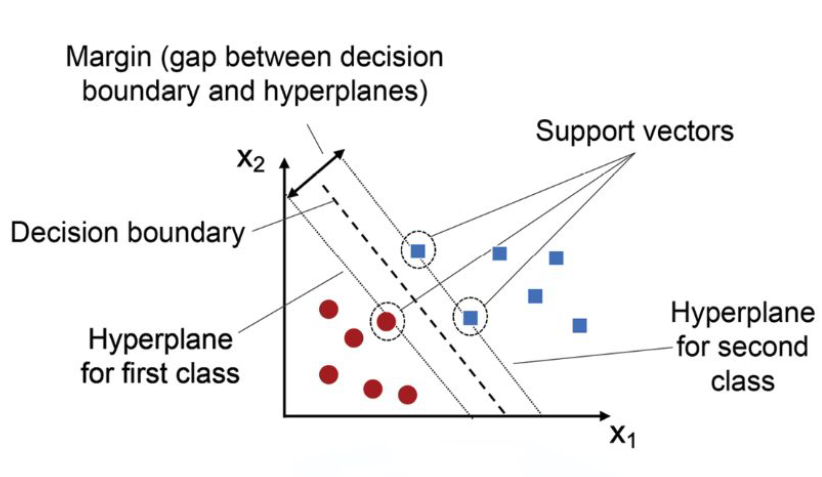
\includegraphics[width=0.75\linewidth]{graphics//chapter3/svm linear.png}
            \caption{SVM in linearly separable class, Source:\cite{gml}}
            \label{fig:svm-linear}
        \end{figure}

        \begin{figure}
            \centering
            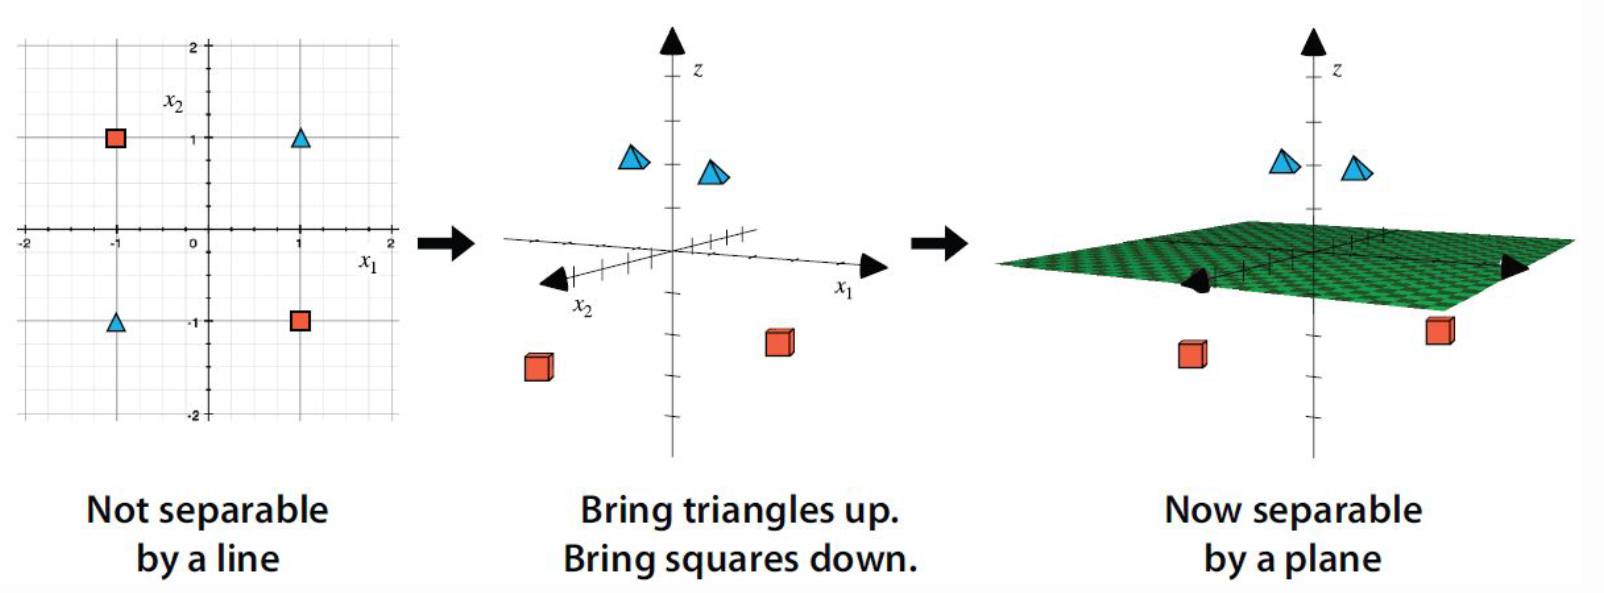
\includegraphics[width=1\linewidth]{graphics//chapter3/svm non linear.png}
            \caption{SVM using Kernel Trick to classify non-linearly separable classes, Source: \cite{gml}}
            \label{fig:svm-nonlinear}
        \end{figure}
        
        SVM chooses the extreme points/vectors that help in creating the hyperplane. These extreme cases are called as support vectors, and hence algorithm is termed as Support Vector Machine.
        
        \subsubsection{K-Nearest Neighbor (KNN)}
        The k-nearest neighbors (KNN) algorithm is a non-parametric, supervised learning classifier, which uses proximity to make classifications or predictions about the grouping of an individual data point. While the KNN algorithm can be used for either regression or classification problems, it is typically used as a classification algorithm, working off the assumption that similar points can be found near one another\cite{knn}.\par \vspace{1em}

        \begin{figure}
            \centering
            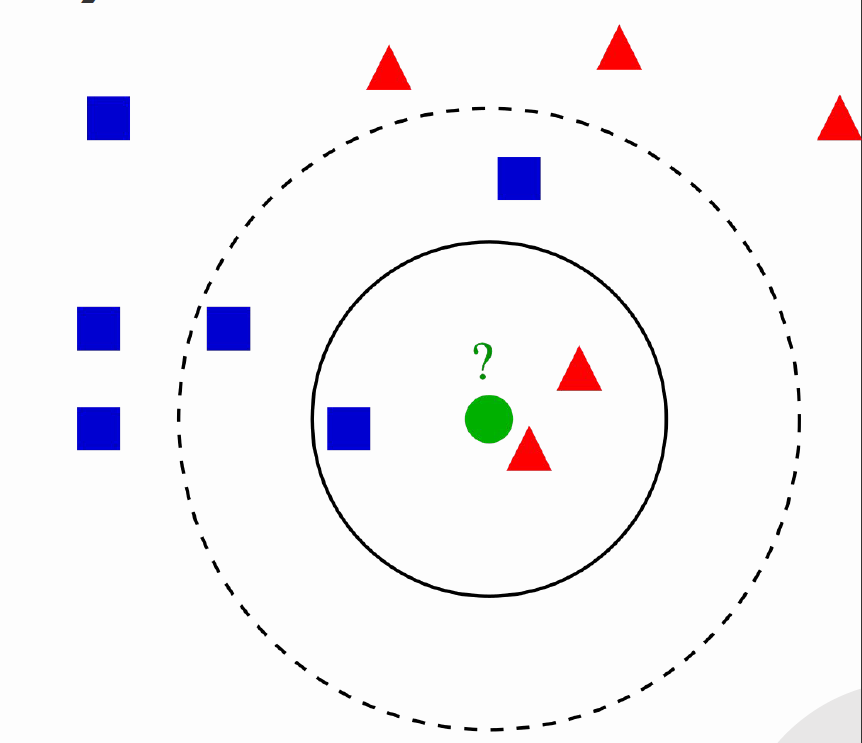
\includegraphics[width=0.75\linewidth]{graphics//chapter3/knn.png}
            \caption[Example of k-NN classification]{Example of k-NN classification. \\The test sample (green dot) should be classified either to blue squares or to red triangles. If k = 3 (solid line circle) it is assigned to the red triangles because there are 2 triangles and only 1 square inside the inner circle. If k = 5 (dashed line circle) it is assigned to the blue squares (3 squares vs. 2 triangles inside the outer circle)\cite{knn-credit}.}
            \label{fig:knn}
        \end{figure}
        
        For classification problems, a class label is assigned on the basis of a majority vote—i.e. the label that is most frequently represented around a given data point is used.
        
        \subsubsection{Ensemble Techniques}
        Ensemble methods use multiple learning algorithms to obtain better predictive performance than could be obtained from any of the constituent learning algorithms alone\cite{em}.\par\vspace{1em}
        
        Supervised learning algorithms perform the task of searching through a hypothesis space to find a suitable hypothesis that will make good predictions with a particular problem. Even if the hypothesis space contains hypotheses that are very well-suited for a particular problem, it may be very difficult to find a good one. Ensembles combine multiple hypotheses to form a (hopefully) better hypothesis. \par\vspace{1em}
        
        Ensemble learning trains two or more Machine Learning algorithms to a specific classification or regression task. The algorithms within the ensemble learning model are generally referred as “base models”, “base learners” or “weak learners” in literature. The base models can be constructed using a single modelling algorithm or several different algorithms. The idea is train a diverse collection of weak performing models to the same modelling task. As a result, the predicted or classified outcomes of each weak learner have poor predictive ability (high bias, i.e. high model errors) and among the collection of all weak learners the outcome and error values exhibit high variance. Fundamentally, an ensemble learning model trains many (at least 2) high-bias (weak) and high-variance (diverse) models to be combined into a stronger and better performing model. Essentially, it’s a set of algorithmic models — which would not produce satisfactory predictive results individually — that get’s combined or averaged over all base models to produce a single high performing, accurate and low-variance model to fit the task as required.\par\vspace{1em}
        
        Ensemble learning typically refers to Bagging (bootstrap-aggregating), Boosting or Stacking/Blending techniques to induce high variability among the base models. Bagging creates diversity by generating random samples from the training observations and fitting the same model to each different sample — also known as “homogeneous parallel ensembles”. Boosting follows an iterative process by sequentially training each next base model on the up-weighted errors of the previous base model’s errors, producing an additive model to reduce the final model errors — also known as “sequential ensemble learning”. Stacking or Blending consists of different base models, each trained independently (i.e. diverse/high variability) to be combined into the ensemble model — producing a “heterogeneous parallel ensemble”. Common applications of ensemble learning include Random Forests (extension of Baggin), Boosted Tree-Models, Gradient Boosted Tree-Models and models in applications of stacking are generally more task-specific — such as combing clustering techniques with other parametric and/or non-parametric techniques. \par\vspace{1em}
        
        \subsubsection{Random Forest}
        
        Random forests or random decision forests is an ensemble learning method for classification, regression and other tasks that operates by constructing a multitude of decision trees at training time. For classification tasks, the output of the random forest is the class selected by most trees. For regression tasks, the mean or average prediction of the individual trees is returned. Random decision forests correct for decision trees' habit of overfitting to their training set.\par\vspace{1em}
        
        \begin{figure}
            \centering
            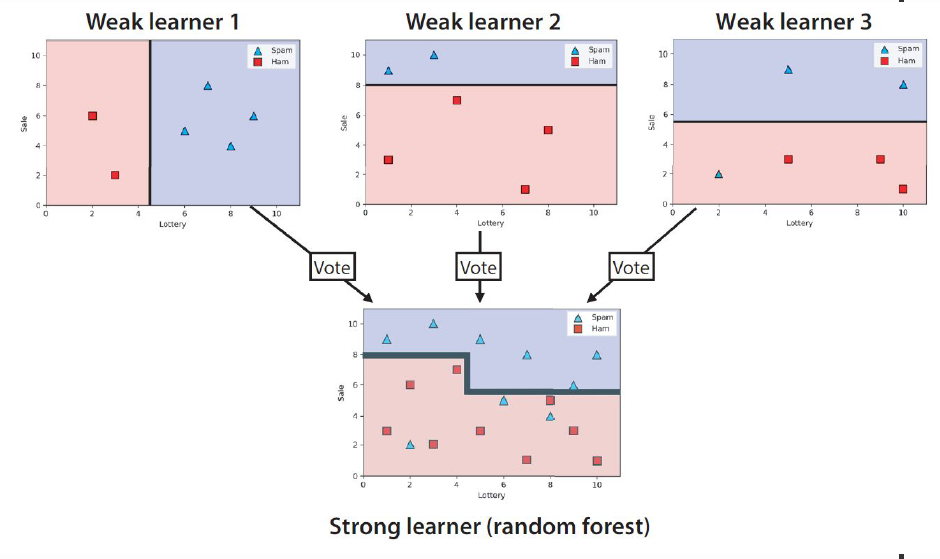
\includegraphics[width=1\linewidth]{graphics//chapter3/random forest.png}
            \caption{Random Forest, Source: \cite{gml}}
            \label{fig:random-forest}
        \end{figure}
        
         Trees that are grown very deep tend to learn highly irregular patterns: they overfit their training sets, i.e. have low bias, but very high variance. Random forests are a way of averaging multiple deep decision trees, trained on different parts of the same training set, with the goal of reducing the variance. This comes at the expense of a small increase in the bias and some loss of interpretability, but generally greatly boosts the performance in the final model\cite{rf-1}\cite{rf-2}.\par\vspace{1em}
        
        \subsubsection{Extreme Gradient Boosting (XGBoost)}   

        \begin{figure}
            \centering
            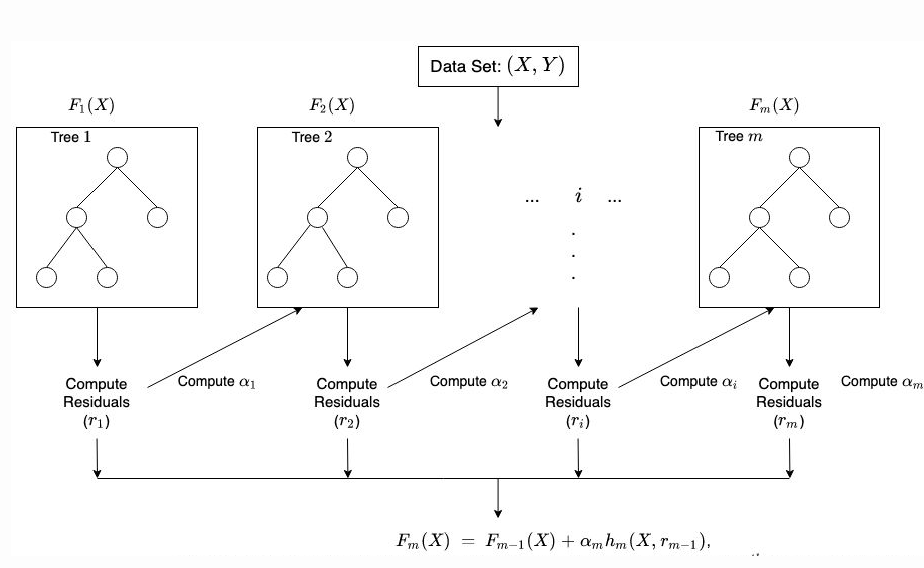
\includegraphics[width=1\linewidth]{graphics//chapter3/xgboost-tree.png}
            \caption{XGBoost Tree, Source: \cite{WEBSITE:xgb-credit-0}}
            \label{fig:xgboost-tree}
        \end{figure}
        
        XGBoost (eXtreme Gradient Boosting) is an advanced implementation of gradient boosting algorithm. It’s a powerful machine learning algorithm especially popular for structured or tabular data. XGBoost has gained fame for its performance in a wide range of machine learning competitions and tasks\cite{xgb}.\par\vspace{1em}
        Since its introduction, this algorithm has not only been credited with winning numerous Kaggle competitions but also for being the driving force under the hood for several cutting-edge industry applications. \par\vspace{1em}
        
        \begin{figure}
            \centering
            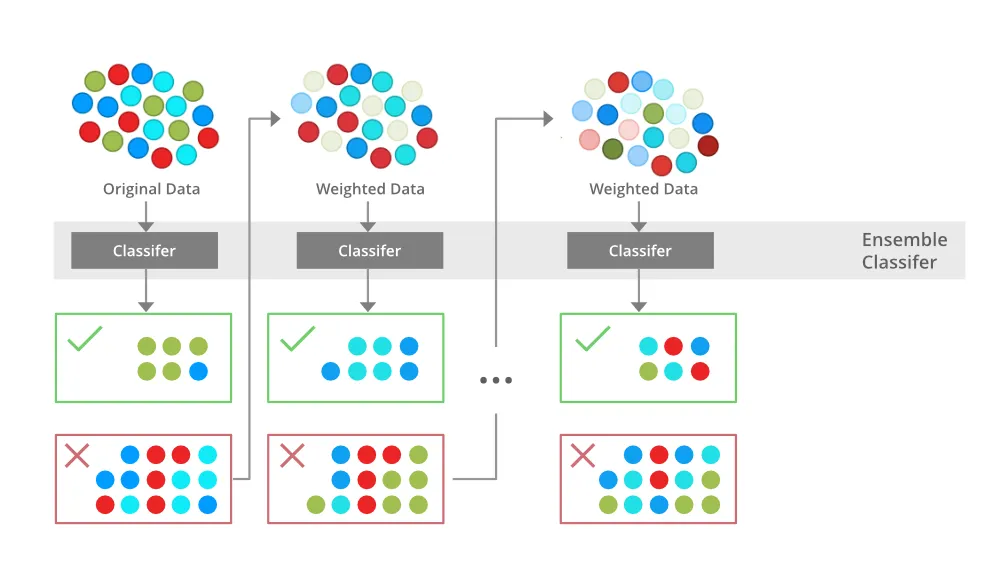
\includegraphics[width=\linewidth]{graphics//chapter3/xgboost1.png}
            \caption{XGBoost Working, Source:\cite{WEBSITE:xgb-credit-1}}
            \label{fig:xgboost-1}
        \end{figure}        

        \textbf{XGBoost Features: }
        \begin{enumerate}
            \item \textbf{Parallelization:} XGBoost approaches the process of sequential tree building using parallelized implementation. This is possible due to the interchangeable nature of loops used for building base learners; the outer loop that enumerates the leaf nodes of a tree, and the second inner loop that calculates the features. This nesting of loops limits parallelization because without completing the inner loop (more computationally demanding of the two), the outer loop cannot be started. Therefore, to improve run time, the order of loops is interchanged using initialization through a global scan of all instances and sorting using parallel threads. This switch improves algorithmic performance by offsetting any parallelization overheads in computation.
            \item \textbf{Tree Pruning:} The stopping criterion for tree splitting within GBM framework is greedy in nature and depends on the negative loss criterion at the point of split. XGBoost uses ‘max\_depth’ parameter as specified instead of criterion first, and starts pruning trees backward. This ‘depth-first’ approach improves computational performance significantly.
            \item \textbf{Hardware Optimization:} This algorithm has been designed to make efficient use of hardware resources. This is accomplished by cache awareness by allocating internal buffers in each thread to store gradient statistics. Further enhancements such as ‘out-of-core’ computing optimize available disk space while handling big data-frames that do not fit into memory.
        \end{enumerate}

        \textbf{Algorithmic Enhancements:}
        \begin{enumerate}
            \item \textbf{Regularization:} It penalizes more complex models through both LASSO (L1) and Ridge (L2) regularization to prevent overfitting.
            \item \textbf{Sparsity Awareness:} XGBoost naturally admits sparse features for inputs by automatically ‘learning’ best missing value depending on training loss and handles different types of sparsity patterns in the data more efficiently.
            \item \textbf{Weighted Quantile Sketch:} XGBoost employs the distributed weighted Quantile Sketch algorithm to effectively find the optimal split points among weighted datasets.
            \item \textbf{Cross-validation:} The algorithm comes with built-in cross-validation method at each iteration, taking away the need to explicitly program this search and to specify the exact number of boosting iterations required in a single run.
        \end{enumerate}

\newpage